\chapter{Introduction}
\section{Overview}
%https://nsdsguidelines.paris21.org/node/291
%https://papers.ssrn.com/sol3/papers.cfm?abstract_id=2622220


%markets:
%https://link.springer.com/article/10.1007/s10551-010-0402-8
%https://www.oecd-ilibrary.org/content/paper/5k49dfg9fb6d-en
%https://www.worldbank.org/en/topic/fragilityconflictviolence/overview

%problem statement/Hook
Between 1990 and 2015, the share of Africans living in absolute poverty fell from 54\% to 41\% \citep{Beegle2019}. However, given the reductions in poverty elsewhere in the world, the proportion of the world's poor who live in Africa has increased in that time period.  Moreover, because of population increase in the continent, this still means that the absolute number of Africans living in poverty has also increased. Just like the reduction in poverty rates hasn't been uniform across continents, the reduction of poverty within Africa hasn't been uniform across countries: the World Bank expects that by 2030, up to two thirds of the world's extremely poor live in Fragile Conflict-affected settings \citep{WorldBank2019}. However, the fact that the global poor are increasingly concentrated in a limited number of countries does not make this a localized issue: instability in one country may have effects throughout the region through increased numbers of refugees and proliferation of armed groups. Such flows may even destabilize countries further away. Climate change is expected to increase this instability further \citep{Burke2009}.

This makes understanding the dynamics of poverty in these countries of crucial importance in reducing poverty worldwide. The constituent papers of this thesis aim to contribute to our knowledge of these dynamics. I present evidence from Sierra Leone, Cameroon and the Democratic Republic of the Congo (DRC).


\section{Theoretical Framework}
HIER MOET EEN OVERGANGS STUKJE KOMEN.

The origins and effects of poverty would be a topic beyond the scope of this thesis. Instead, each chapter in this thesis explores a different aspect of the larger problem. In doing this I limit my focus on three sources of risks and opportunities for development, the effect of which on development outcomes is modulated by social capital and institutions, as outlined in Figure \ref{intro:fig:framework}. 

 (see Figure \ref{intro:fig:framework}).

\begin{figure}[htb]
  \centering
  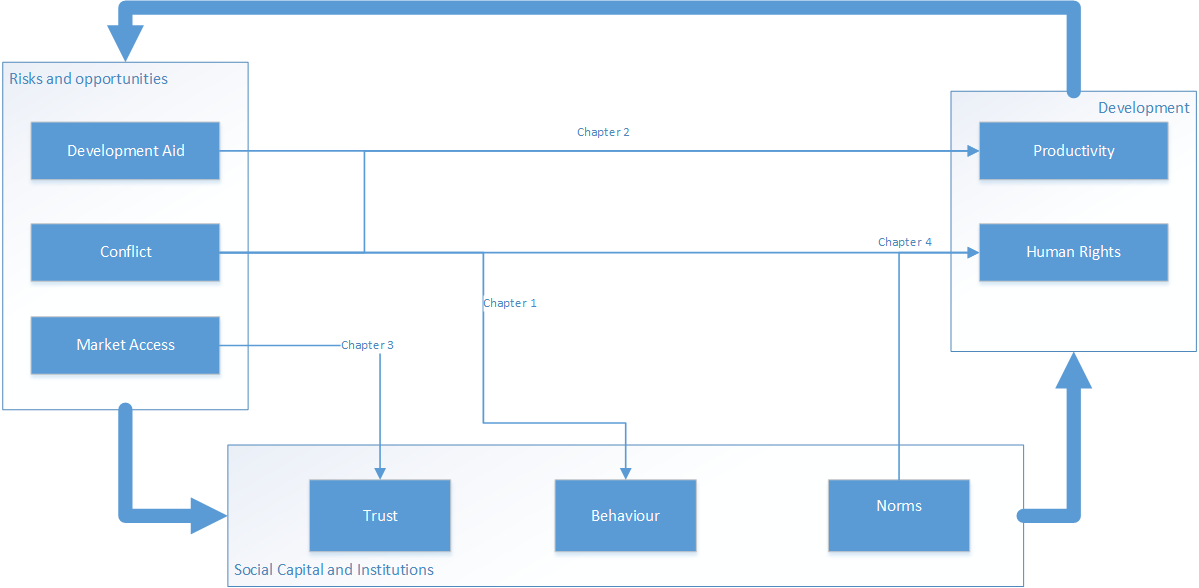
\includegraphics[width=0.8\linewidth]{"\git/thesis/analysis/introduction/figures/conceptual_framework.png"}
  \caption{Conceptual Framework}
  \label{intro:fig:framework}
\end{figure}

\subsection{Risks and Opportunities}\
As for the risks and opportunities to development I consider, the first is violent conflict. \citet{Collier2003} has labelled conflict ``Development in Reverse'', clearly indicating the risk conflicts poses to development. The 2011 World Development Report was titled Conflict, Security, and Development, further underscoring the importance of violent conflict poses in shaping development outcomes \citep{WorldBank2011}. Aside from the human rights violations that are inherent to violent conflict, other consequences include: decreased economic activity \citep{Collier1999} deforestation \cite[e.g.][]{Connectiona}, long-term incidence of domestic violence \citep[e.g.][]{LaMattina2017, Muller2019}, (mental) health problems \cite[e.g.][]{Smith2002, Iqbal2006a,Akresh2011} and food insecurity \cite[e.g.][]{Lecoutere2005, Verwimp2012}. However, some effects which may have some benefit to long-term development have been described, such as increased collective action \citep{Bellows2009b}, political participation \citep{Blattman2009a} and increased pro-social behaviour \citep{Voors2012a}.

Next, I consider an opportunity for development: markets \todo{text flow}. Markets provide opportunities for exchange and specialization, which can boost economic development. At the national level, trade is seen as a promising way to increase productivity in developing economies. Dutch development aid, for example, has a large focus on the complementarities between trade and development as a way of increasing investments and thus productivity \citep[see e.g.][]{Zoomers2014}. Aside these impacts on the national level, increased access to markets have been shown to have effects at the local and individual level as well: markets are associated with trust \citep{Tu2010,Fischer2008}; increased rationality \citep{List2008,Cecchi2013,Braga2009} and decreases in risk aversion \citep{Melesse2015}. This corresponds with findings that from large-scale societies (which include markets) engage more in pro-social behaviour \cite{Henrich2005,Henrich2010}. These national and individual effects make that markets are an important consideration in analysing the development process.


%put in for development aid vs institutional reform: https://www.aeaweb.org/articles/pdf/doi/10.1257/jel.44.4.973
Thirdly, I consider development aid. At the turn of the century, the Millennium Development Goals were adopted in the hopes that the world's poorest countries (particularly in Africa) could be lifted out of poverty with a large-scale international effort. The underlying assumption was that a core challenge to African economies were adverse geographical conditions which hinder growth; ambitious invenstments by the international development community could then help increase agricultural productivity and decrease the impact of tropical diseases \todo{kies wat dingen van Sachs hier}. However, concurrently there was doubt about development aid's capability to achieve growth that reached the poorest. \citet{Easterly2007} labels Development Assistance a ``mistake'', claiming that ``we don't know what actions achieve development''. \todo{dat rodirk paper wat hierboven staat past hier ook wel} A large literature has since sprung up that aims to fill exactly that knowledge gap and find out which development interventions work, and which don't. Improvements in statistical techniques and data collection methods have allowed development economists to get more accurate assessments of the impact of aid programs. Academics and development NGOs have embraced methods such as Randomized Controlled Trials (RCTs) to find out what works and what doesn't \todo{CITE}.   


\subsection{Social Capital and Institutions}
The impact that these risks and opportunities can have differs across countries. Some countries have been better able to exploit the advantages markets offer than others; some conflicts have larger consequences than others \todo{dan dit zonder herhaling?}. The key factor that sets apart countries that are succesful in avoiding risk and copitalizing on opportunities is, is their institutional environment \citep{Rodrik2004,Acemoglu2000}. This term is used to describe the rules and norms that shape (economic) life. It covers crucial things such as protection of property rights and equal treatment by the law \citep{Acemoglu2005}. Such good institutions  foster development by incentivizing innovation. However, the relationship between institutions and development does not run in one direction. While institutions cause growth \citep{Acemoglu2000}, the economic growth that accompanies development also allows for better institutions. It is possible that countries could enter a virtuous cycle, where improved institutional quality enhances growth, which improves institutional quality \citep{Voors2011}.

%
Social capital is closely related to institutions. \todo{define social capital} Especially in poorer countries, social capital plays an important role in facilitating economic activity \citep{Knack1997}. In such countries, social capital may be a substitute for formal institutions by providing insurance and securing property rights. To a large extent, such social capital is underpinned by pro-social behaviour. \todo{really?}

%However, institutions can also increase cooperative behaviour \citep{Bo2008,Henrich2010}. 
This implies that countries with a high level of social capital or good institutions can enter a virtuous cycle of institutions producing growth and social capital; and social capital and growth producing quality institutions. The question on how to enable such a virtuous cycles for fragile states is too large for any one thesis. This thesis aims to provide empirical, micro-level level evidence on how social capital and behaviour mediate development in fragile states. Figure \ref{intro:fig:framework} outlines these concepts. Each chapter in this thesis then explores one subset of the possible relationships within the framework.

\subsection{Development}
As for development, I focus on agricultural productivity and human rights. I focus on agricultural production, as the poorest of the world often depend on subsistence agriculture. Furthermore, agricultural productivity is seen as a necessary precondition for further, economy-wide, productivity improvements. \todo{why?} 

However, a focus on productivity is too narrow to fully capture the problems that life in fragile states presents in terms of development. Productivity gains mean little in the face of widespread human rights violations. Human dignity is a crucial part of development.


\section{Research Questions}
The questions this thesis aims to answer are:
\begin{enumerate}
	\item What is the relationship between conflict and competitive behaviour? (Chapter \ref{chap:slfootball});
	\item What is the effect of input subsidies on novel technology adoption? (Chapter \ref{chap:n2a_impact});
	\item What is the effect of market access on trusting behaviour (Chapter \ref{chap:cameroontrust}); and,
	\item What are the drivers of sexual and gender-based violence in Eastern Congo (Chapter \ref{chap:congogbv}).
\end{enumerate}

\section{Contribution}
The primary contribution of this thesis lies in the collection of large-scale datasets in settings where little micro-level data has been collected due to the difficulties in doing so; either because they are remote, like Eastern Sierra Leone and Northern Cameroon, or because of conflict, like Eastern DRC. This fits within a broader trend where the amount of data collected in such states has increased over the past decades, in part because of increased efforts to evaluate development aid in such settings. The primary funding for this PhD-thesis comes from such an evaluation: the MFS II evaluations, commissioned by the Dutch ministry of foreign affairs.

Despite this increase in data collection efforts, citizens of Fragile States remain under-represented in studies on behaviour. Chapter \ref{chap:slfootball} contributes by studying the effects of conflict on youth in Sierra Leone. Chapter \ref{chap:cameroontrust} contributes to this by collecting large-scale data on behaviour of an understudied group: Africans from rural areas, with poor access to markets. Chapter 4 studies the dynamics of sexual violence in Congo. Despite the prominence the topic has had in public discourse on Congo, and despite its severity, little data exists on these dynamics. This is partly due the difficulties and costs inherent in operating in unstable countries.

All data sets used for analyses, and all protocols and analysis scripts are released to the public domain.


\section{Outline}


%bibliography, this is needed for bibtex
\clearpage 
\bibliographystyle{chicago}
%path to .bib file (e.g. automatically exported by mendeley) DO NOT include the file extension!
\bibliography{\onedrive/Literatuur/Bibtex/Thesis}